\subsection{Implementation}

Our implementation of \system{} includes relays, an oracle, and 
a client. \system{} is open source.  \system{} is currently deployed globally, and
any user may use it today.\footnote{We have released an anonymized source code repository,
complete with usage instructions, at: \url{https://bitbucket.org/ransom_research/ran/}}

We assume that users and machines are trustworthy, and therefore the system runs 
securely.  This implementation of \system{} allows a client to avoid a single country 
at a time; attacks on \system{}, such as Denial of Service attacks and targetted 
surveillance of the relays, are outside the scope of the paper.

\paragraph{Relays.}  The current deployment has ten relays, one in each
of the following
countries: Brazil,  Germany, Singapore, Japan, Australia, France, United
States, United Kingdom, Netherlands, and Canada; Figure~\ref{fig:relay_locations}
shows these relay locations, along with their corresponding ASes. These relays operate
as Ubuntu Virtual Private Servers (VPSes) with Squid as the proxy
server and the \system{} Relay software.

\begin{figure}[t!]
\centering
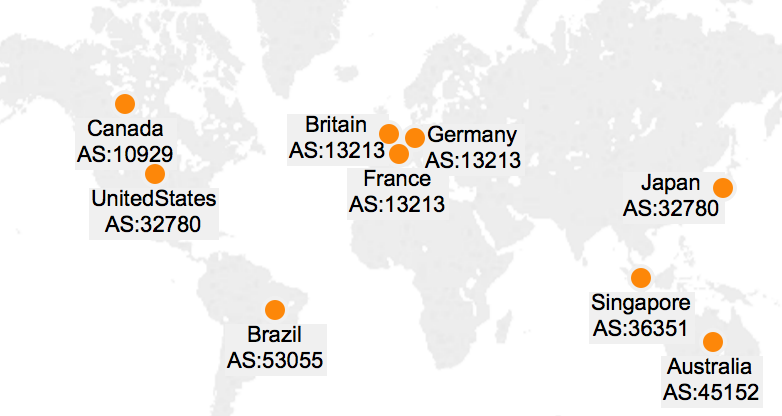
\includegraphics[width=.4\textwidth]{relay_map}
\caption{The locations and ASNs for \system{} relays.}
\label{fig:relay_locations}
\end{figure}

\paragraph{Oracle.}  The oracle software runs on a Fujitsu RX200 S8 server with dual, 
eight-core 2.8~GHz Intel Xeon E5 2680 v2 processors with 256GB RAM running 
RedHat Linux. 

\paragraph{Client.} To evaluate the \system{} deployment, we set up a client 
machine in the Netherlands, which simply accesses web content and uses the PAC 
file generated by the oracle. 
